\documentclass[a4paper]{article}

\usepackage[margin=1.2in]{geometry}
\usepackage{graphicx}
\usepackage{amsmath,amssymb,amsthm,bm}
\usepackage{latexsym,color,minipage-marginpar,caption,multirow,verbatim}
\usepackage{enumerate}
\graphicspath{ {./Users/omerronen/Documents/Phd/stat210A/} }
\usepackage{float}

\newcommand{\RR}{\mathbb{R}}
\newcommand{\PP}{\mathbb{P}}
\newcommand{\EE}{\mathbb{E}}

\newcommand{\cP}{\mathcal{P}}
\newcommand{\cC}{\mathcal{C}}
\newcommand{\cX}{\mathcal{X}}

\newcommand{\ep}{\varepsilon}

\newcommand{\simiid}{\overset{\textrm{i.i.d.}}{\sim}}
\newcommand{\simind}{\overset{\textrm{ind.}}{\sim}}

\begin{document}

\title{Stats 215A, Fall 2020\\
  Homework 3\\}
\date{}
\maketitle
\vspace{-5em}
\section{EM Algorithm}
\begin{enumerate}
\item Our observed data is the $X$ vector the latent variable is the cluster assignment which we'll denote $Z$ with $z_i\sim\text{Ber}(\pi)$. The joint likelihood is
\[
L(X,Z;\theta) = \prod_{i=1}^{n} \left(\pi f_{\mu_{0}}(x_i)\right)^{z_i} \cdot \left((1-\pi) f_{\mu_{1}}(x_i)\right)^{1-z_i}
\]
The vector of model parameters is $\theta = (\pi, \mu_1, \mu_2)$
It is also interesting to note that using bayes theorem 
\[
\begin{aligned}
\mathbb{P} (z_i=1|X, \theta) &= \frac{\pi f_{\mu_{0}}(x_i)\cdot \mathbb{P}(X_{(-i)})}{\pi f_{\mu_{0}}(x_i)\cdot \mathbb{P}(X_{(-i)}) + (1-\pi) f_{\mu_{1}}(x_i)\cdot \mathbb{P}(X_{(-i)})}\\
&= \frac{\pi f_{\mu_{0}}(x_i)}{\pi f_{\mu_{0}}(x_i) + (1-\pi) f_{\mu_{1}}(x_i)}
\end{aligned}
\]
Which defines the conditional distribution of $Z$ given $X$ and $\theta$
\item The E step we take the conditional expectation of the log-likelihood given our current estimate of the parameters over $Z$
\[
\begin{aligned}
\mathbb{E}_{Z|X,\theta^{(t)}} \log (L(X,Z;\theta)) &= 
\mathbb{E}_{Z|X,\theta^{(t)}} \sum_{i=1}^{n} z_i \log(pi f_{\mu_{0}}(x_i)) + (1-z_i)\log((1-pi) f_{\mu_{1}}(x_i))\\
&= \sum_{i=1}^{n} t_i^{(t)} \log(\pi f_{\mu_{0}}(x_i)) + (1-t_i^{(t)})\log((1-\pi) f_{\mu_{1}}(x_i))\\
&= \sum_{i=1}^{n} t_i^{(t)} (\log(\pi)+ \log(f_{\mu_{0}}(x_i))) + (1-t_i^{(t)})(\log((1-\pi))+ \log(f_{\mu_{1}}(x_i)))
\end{aligned}
\]
With $t_i^{(t)} = \mathbb{P} (z_i=1|X, \theta^{(t)}) $.\\
What we actually do in the E step is update $t_i^{(t-1)}$ to $t_i^{(t)}$, it'll be clear why after we derive the M step formula.
\item On the M step we maximize the expected likelihood with respect to the parameters
\[
\frac{\partial}{\partial\pi}\mathbb{E}_{Z|X,\theta^{(t)}} \log (L(X,Z;\theta)) =  \sum_{i=1}^{n} t_i^{(t)} (\frac{1}{\pi})- (1-t_i^{(t)})(\frac{1}{1-\pi})
\]
Finding the roots of the equation we have
\[
\pi^{(t+1)} = \frac{\sum_{i=1}^{n}t_i^{(t)}}{n}
\]
Next we move to the estimation of $\mu_0,\mu_1$
\[
\frac{\partial}{\partial\mu_0}\mathbb{E}_{Z|X,\theta^{(t)}} \log (L(X,Z;\theta)) = 
\sum_{i=1}^{n} t_i^{(t)} \frac{x_i}{\mu_0} -n
\]
Finding the roots of the equation we have
\[
\mu_0^{(t)} = \frac{\sum_{i=1}^{n} t_i^{(t)} x_i}{n}
\]
and using identical calculations we have
\[
\mu_1^{(t)} = \frac{\sum_{i=1}^{n} (1-t_i^{(t)}) x_i}{n}
\]
\item Poisson data
\begin{figure}[H]
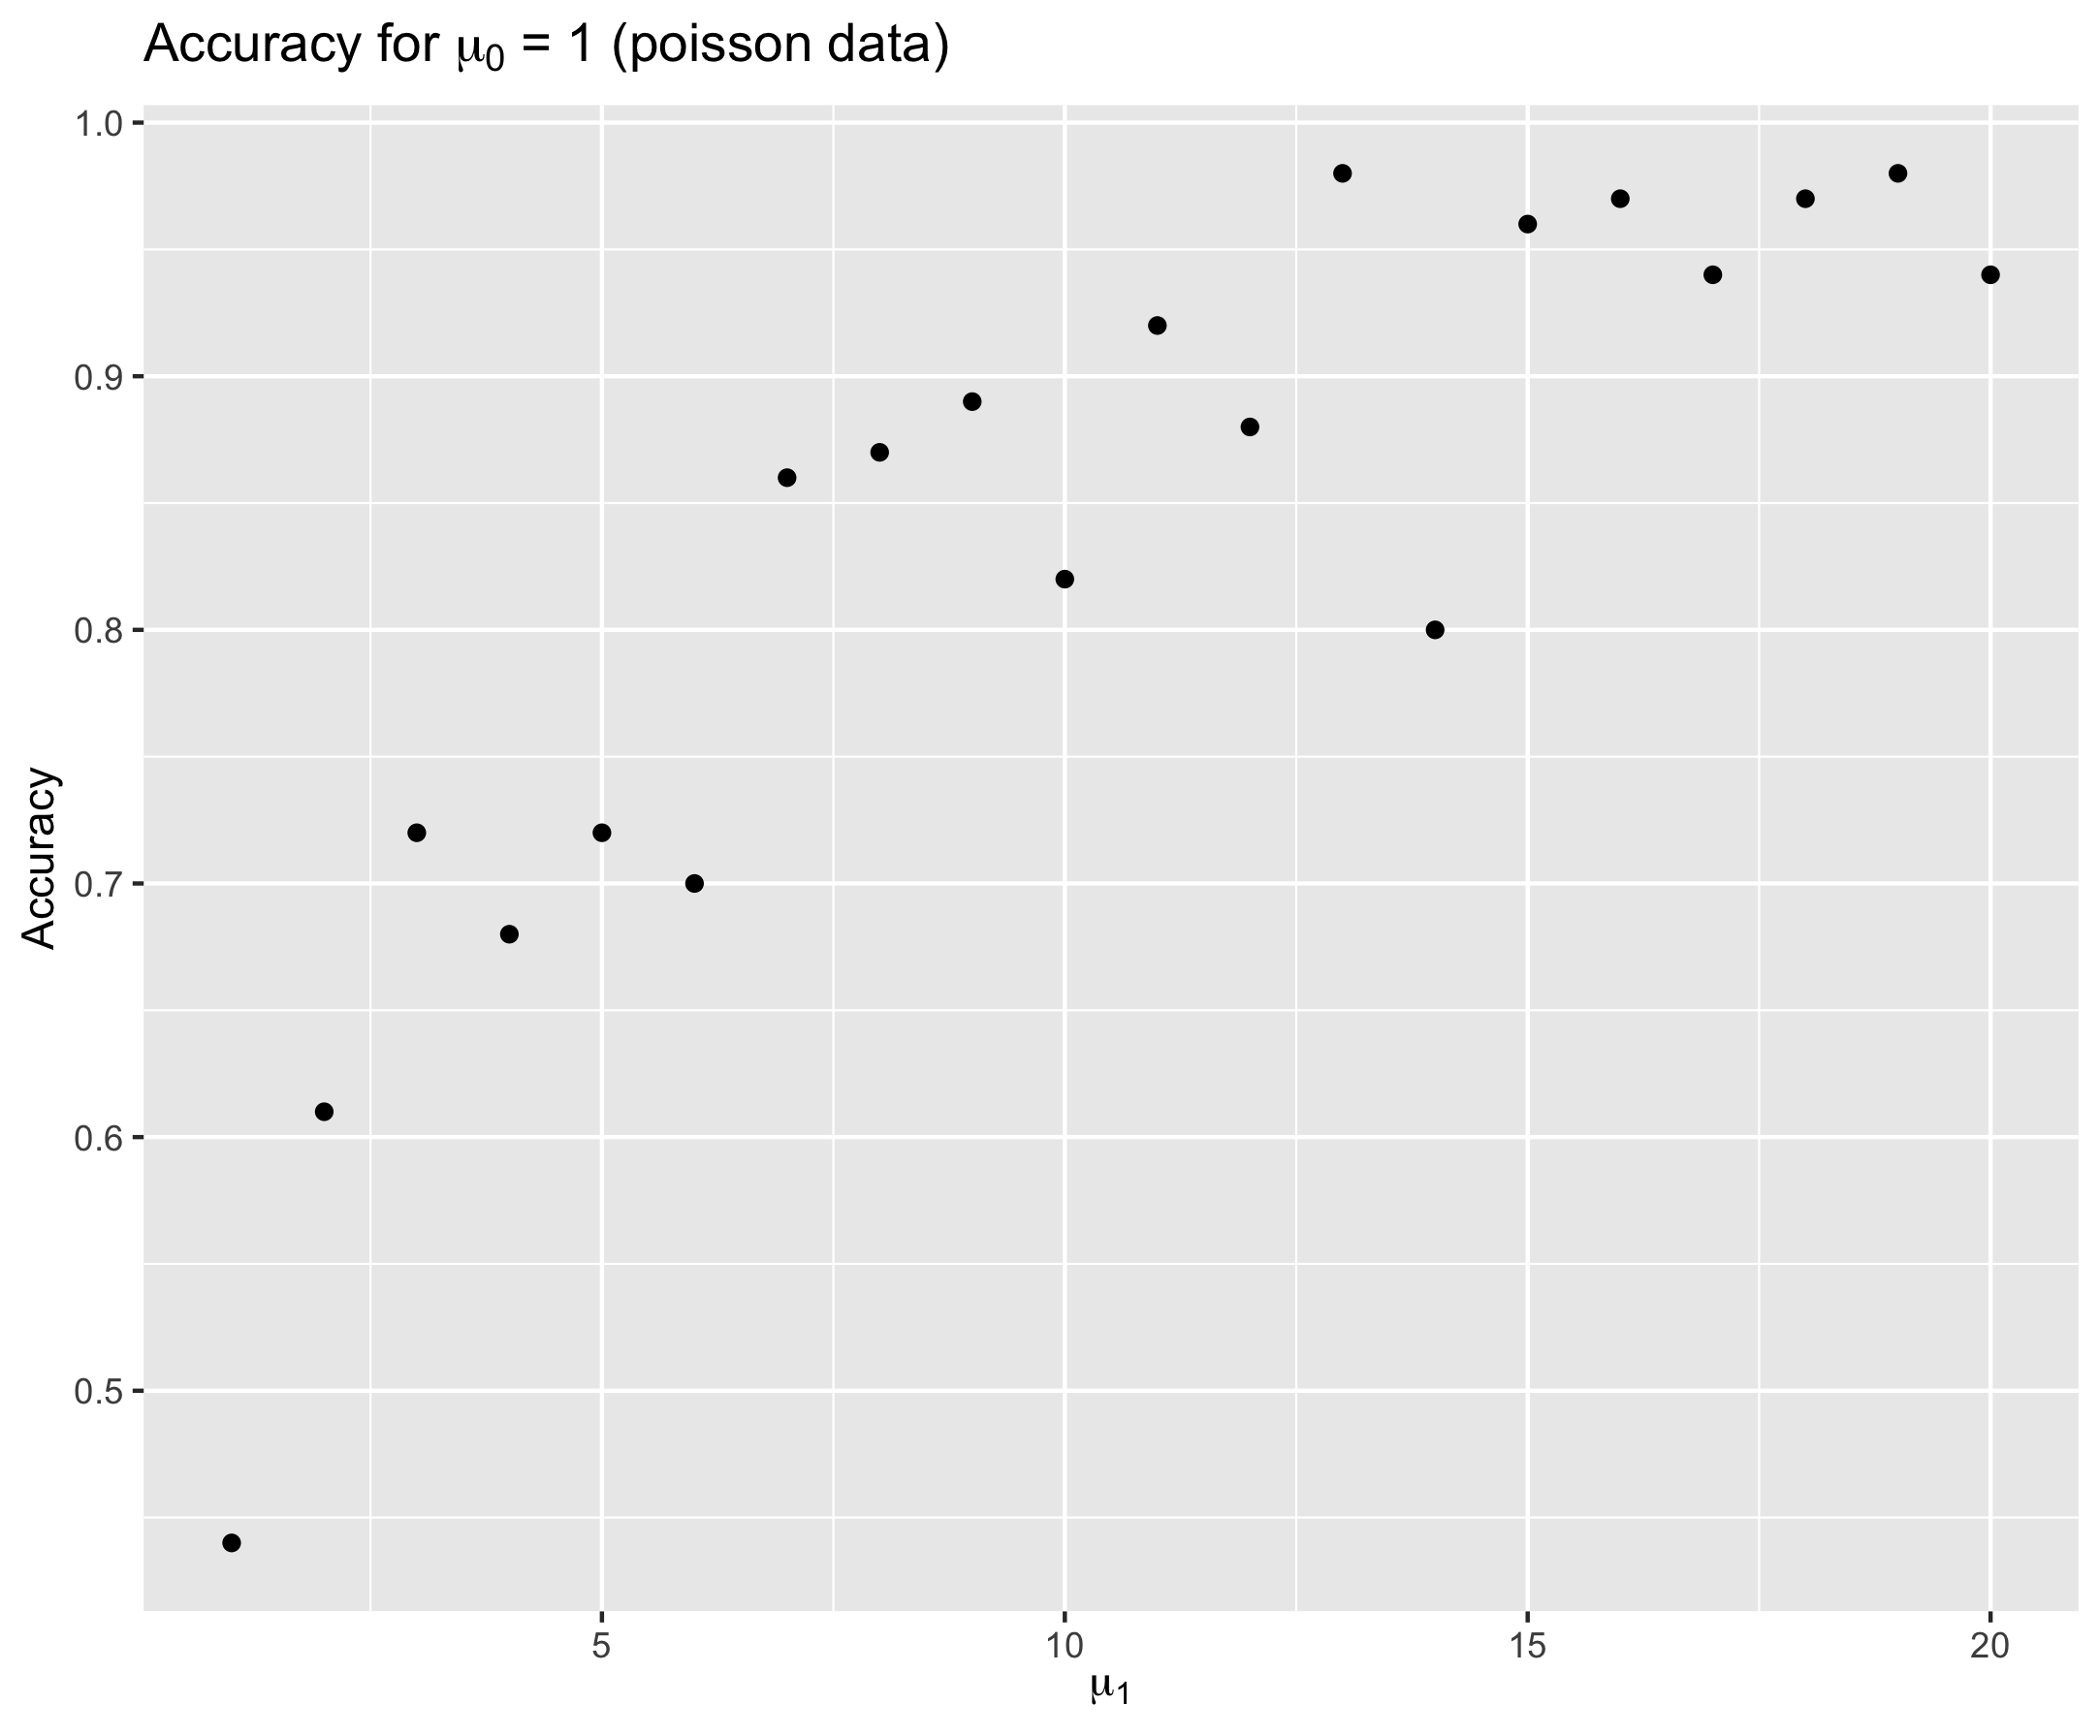
\includegraphics[scale=0.15]{pois.png}
\end{figure}
\item Binomial data
\begin{figure}[H]
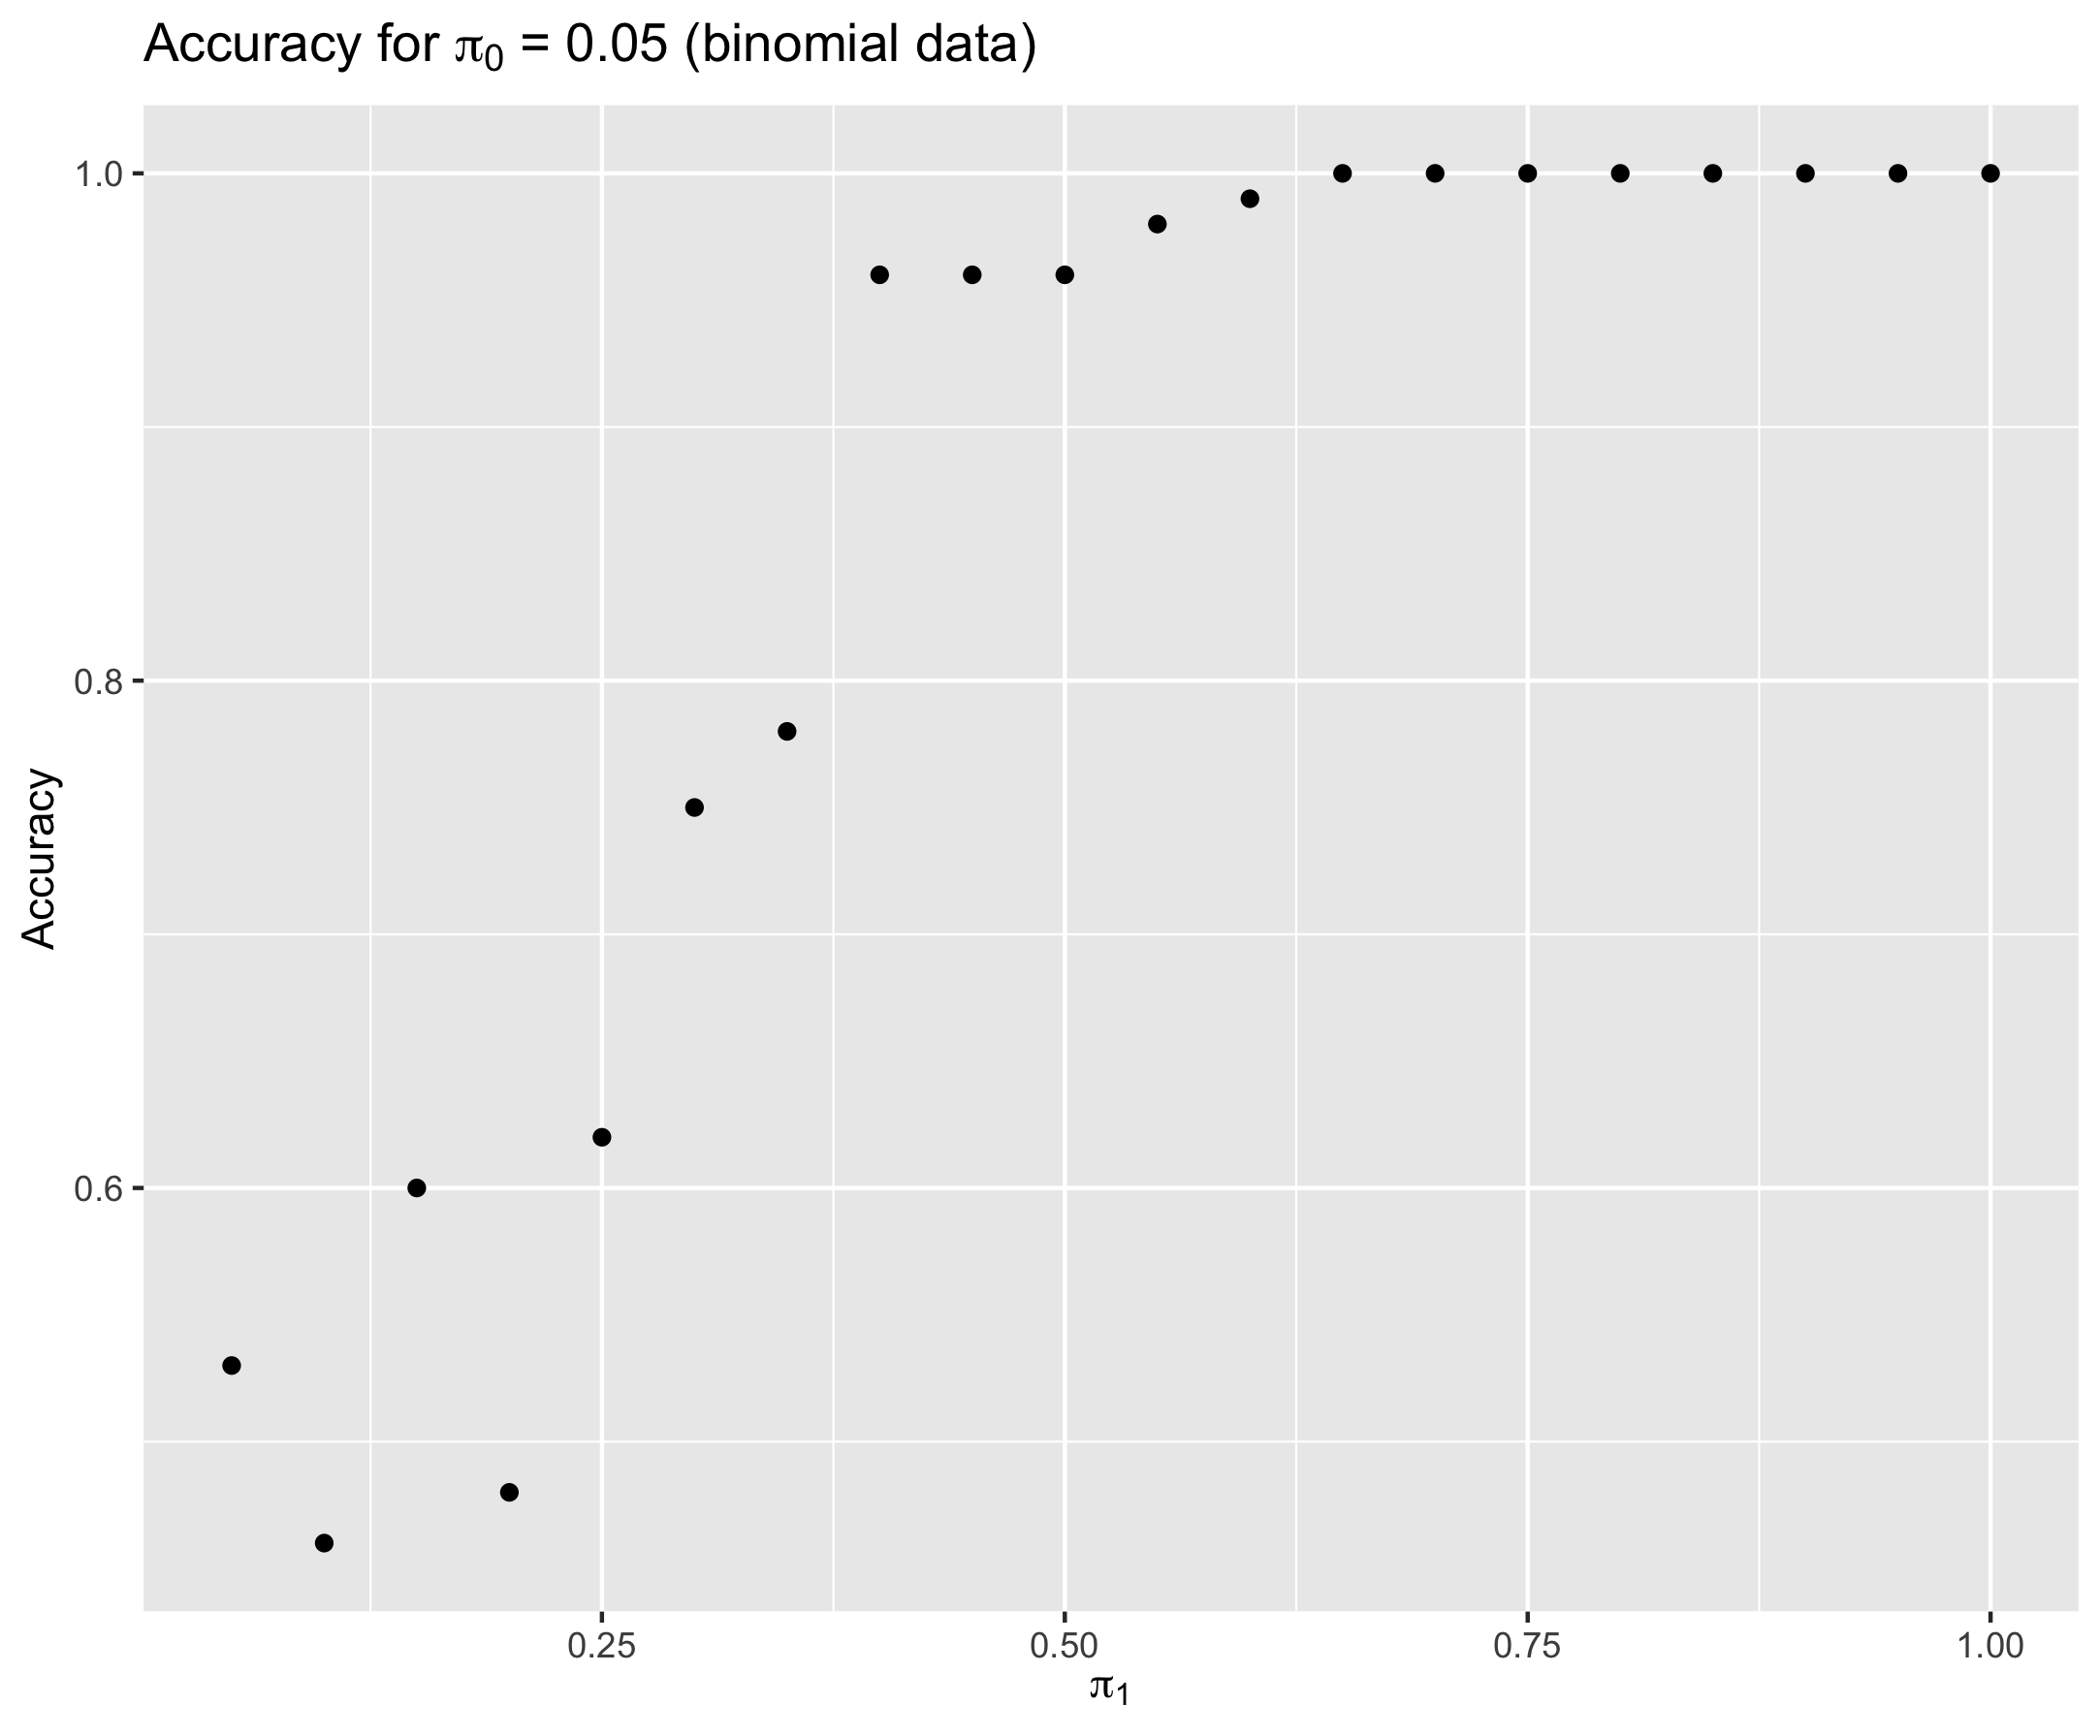
\includegraphics[scale=0.15]{binom.png}
\end{figure}
\end{enumerate}
\end{document}